\documentclass[sigconf]{acmart}

\usepackage{amsmath}
\let\Bbbk\relax
\usepackage{amssymb}
\usepackage{amsfonts}
\usepackage{booktabs}
\usepackage{graphicx}
\usepackage{microtype}
\usepackage{algorithm}
\usepackage{algorithmic}
\usepackage{subcaption}
\usepackage{tikz}
\usepackage{pgfplots}
\pgfplotsset{compat=1.18}

%% Rights management information.
\setcopyright{acmlicensed}
\acmConference[ICIIT 2027]{9th International Conference on Intelligent Information Technology}{February 2027}{Singapore}
\acmYear{2027}
\acmDOI{10.1145/XXXXXX.XXXXXX}
\acmISBN{978-1-4503-XXXX-X/27/02}

\setlength{\textfloatsep}{6pt plus 1pt minus 2pt}
\setlength{\floatsep}{5pt plus 1pt minus 1pt}
\setlength{\intextsep}{5pt plus 1pt minus 1pt}
\setlength{\abovecaptionskip}{2pt plus 1pt minus 1pt}
\setlength{\belowcaptionskip}{1pt plus 1pt minus 1pt}
\setlength{\bibsep}{0.2pt plus 0.1pt minus 0.1pt}

\begin{document}

\title{Optimizing Programmatic Ad Spend Pacing via Multi-Horizon Temporal Fusion Transformers}

\author{Maik Nguyen}
\affiliation{%
  \institution{School of Computing, National University of Singapore}
  \city{Singapore}
  \country{Singapore}
}
\email{maik.nguyen@u.nus.edu}

\begin{abstract}
Programmatic real-time bidding (RTB) under finite budget constraints requires demand-side platforms (DSPs) to dynamically regulate expenditure pacing across heterogeneous multi-day horizons. In modern advertising exchanges, the systemic transition from Generalized Second-Price (GSP) to First-Price Auctions (FPA) has eliminated the clearing price buffer, exposing advertisers directly to the ``winner's curse'' and amplifying the penalty for sub-optimal pacing. Conventional pacing heuristics---ranging from Uniform Linear Pacing (ULP) to Proportional-Integral-Derivative (PID) feedback controllers---frequently incur premature budget exhaustion or severe under-delivery under auction volatility. In this paper, we propose an end-to-end, multi-horizon ad spend pacing framework powered by Temporal Fusion Transformers (TFT) that unifies budget control across both First-Price and Second-Price auction regimes. Our architecture couples Gated Residual Networks (GRN) to stabilize gradients, Variable Selection Networks (VSN) to filter auction micro-jitter, and Interpretable Multi-Head Attention to isolate cyclic diurnal and weekly patterns over a 168-hour lookback. We incorporate the multi-quantile trajectory forecasts $\hat{y}_{t+\tau}(q)$ ($q \in \{0.1, 0.5, 0.9\}$) across a 24-hour planning horizon into a closed-form throttling policy that dynamically rescales outgoing bid prices, and prove its downside solvency bound under both FPA and GSP mechanics. Furthermore, we develop a dual-boundary spike detector that decouples exogenous market shocks from expected diurnal peaks. Comprehensive empirical evaluations on the iPinYou global RTB benchmark across 19.5 million auctions demonstrate that our approach achieves an out-of-sample MASE of $0.1583$, decisively outperforming seasonal naive persistence across full 24-hour horizons. Economically, it delivers $94.65\%$ budget utilization without premature budget depletion ($0.0\%$) and suppresses pacing volatility to $0.0765$ (over $53\%$ smoother than PID feedback control at $0.1655$), establishing a new state-of-the-art for programmatic budget control.
\end{abstract}

\begin{CCSXML}
<ccs2012>
   <concept>
       <concept_id>10002951.10003227.10003447</concept_id>
       <concept_desc>Information systems~Computational advertising</concept_desc>
       <concept_significance>500</concept_significance>
       </concept>
   <concept>
       <concept_id>10010147.10010257.10010293.10010294</concept_id>
       <concept_desc>Computing methodologies~Neural networks</concept_desc>
       <concept_significance>500</concept_significance>
       </concept>
   <concept>
       <concept_id>10002950.10003648.10003688</concept_id>
       <concept_desc>Mathematics of computing~Time series analysis</concept_desc>
       <concept_significance>300</concept_significance>
       </concept>
 </ccs2012>
\end{CCSXML}

\ccsdesc[500]{Information systems~Computational advertising}
\ccsdesc[500]{Computing methodologies~Neural networks}
\ccsdesc[300]{Mathematics of computing~Time series analysis}

\keywords{Programmatic Advertising, Real-Time Bidding, Demand-Side Platforms, Budget Pacing, Temporal Fusion Transformers, Multi-Horizon Forecasting, Quantile Loss, Spike Detection}

\maketitle

\section{Introduction}
Real-time bidding (RTB) has become the dominant paradigm for modern digital advertising, processing billions of ad impressions daily~\cite{zhang2014real}. Historically, programmatic ad exchanges relied almost exclusively on Generalized Second-Price (GSP) auctions~\cite{lee2013real}. However, over the past decade, major programmatic exchanges have overwhelmingly transitioned to First-Price Auctions (FPA) to ensure pricing transparency amidst header bidding~\cite{despotakis2021first,zhou2021bid}. In second-price auctions, an aggressive bid is cushioned by the second-highest bid; in first-price auctions, winning bidders pay their exact bid price. This fundamental market shift removes the second-price clearing cushion, creating acute vulnerability to the ``winner's curse'' if pacing fails.

In contemporary Demand-Side Platforms (DSPs), real-time bidding is therefore decoupled into two distinct, cooperative operational layers:
\begin{enumerate}
    \item \textbf{Micro-Level Bid Shading:} At millisecond scale per impression, a predictive model shades raw valuations to maximize immediate surplus against competitive clearing distributions~\cite{zhou2021bid,balseiro2021budget}.
    \item \textbf{Macro-Level Budget Pacing:} At hourly intervals, a pacing governor regulates aggregate expenditure velocity across the multi-day campaign lifespan $T$ to satisfy monetary budget $B$~\cite{xu2015smart,grigas2017profit}.
\end{enumerate}
Without robust macro-pacing, an unconstrained bidding policy rapidly exhausts its budget during early morning or midday traffic peaks, leaving the campaign inactive during high-converting evening hours. Conversely, overly conservative bidding risks severe under-delivery, forfeiting reach and failing to utilize allocated capital~\cite{bhalgat2012online}. In first-price auctions, this tension is exacerbated: because spend is directly proportional to submitted bids, pacing volatility translates instantly into balance-sheet exposure without an absorbing buffer.

Despite widespread industry need, classical pacing mechanisms display critical structural limitations:
\begin{enumerate}
    \item \textbf{Uniform Linear Pacing (ULP):} Allocates a constant nominal velocity $B/T$ to each discrete interval. This heuristic fundamentally ignores predictable diurnal circadian rhythms and weekend traffic shifts~\cite{xu2015smart}.
    \item \textbf{Feedback Control (PID):} Adjusts bid multipliers reactively based on accumulated spending error. While simple, PID controllers suffer from phase lag, phase margin instability, and severe overshoot when sudden auction spikes occur~\cite{lee2013real}.
    \item \textbf{Lagged Tree-based Regressors (GBDT):} Autoregressive models (e.g., LightGBM) fail to capture multi-horizon joint dependency structures and produce point estimates that lack calibrated uncertainty bounds~\cite{ke2017lightgbm}.
\end{enumerate}

To overcome these deficiencies, we formulate ad spend pacing as an end-to-end multi-horizon time series forecasting problem integrated with a risk-averse control policy that unifies First-Price and Second-Price auction mechanisms. We introduce a pacing framework leveraging \textbf{Temporal Fusion Transformers (TFT)}~\cite{lim2021temporal}. By explicitly ingesting static campaign metadata, historical auction time series, and known future calendar indicators, TFT models non-linear dynamics while isolating interpretable temporal dependencies. Crucially, TFT outputs calibrated multi-quantile predictions ($\hat{y}_{t+\tau}(0.10), \hat{y}_{t+\tau}(0.50), \hat{y}_{t+\tau}(0.90)$), enabling our downstream throttling policy to hedge against downside auction volatility.

The principal contributions of this work are summarized as follows:
\begin{itemize}
    \item \textbf{Unified Auction Pacing Framework:} We formulate a macro-pacing architecture that operates seamlessly across both modern First-Price (FPA) with micro bid shading and Generalized Second-Price (GSP) auctions, eliminating the reliance on second-price market cushions.
    \item \textbf{Multi-Horizon TFT Architecture:} We model campaign expenditure over a 24-hour horizon with a 168-hour (7-day) lookback window, utilizing Gated Residual Networks (GRN) to suppress gradient vanishing and Variable Selection Networks (VSN) to filter auction micro-jitter.
    \item \textbf{Quantile-Hedging Throttling Policy \& Solvency Proof:} We design a closed-form bid multiplier $\alpha_{t+1}$ anchored to the cumulative 90th-percentile spend forecast $\sum \hat{y}(0.90)$, mathematically proving downside budget solvency under both FPA and SPA regimes.
    \item \textbf{Dual-Boundary Spike Detection:} We introduce an adaptive shock detector that contrasts realized spend against the TFT conditional median $\hat{y}_t(0.50)$ and 90th percentile $\hat{y}_t(0.90)$, robustly decoupling exogenous market shocks from expected diurnal peaks.
    \item \textbf{Empirical Rigor on Global RTB Benchmark:} Evaluating on 19.5 million iPinYou auctions across a strict 60-day train, 15-day validation, and 15-day test chronological split, our model achieves a superior MASE of $0.1583$, $94.65\%$ budget utilization, $0.0\%$ premature exhaustion, and a smooth PVI of $0.0765$ (a $>53\%$ volatility reduction over PID control).
\end{itemize}

\section{Problem Formulation \& System Model}

\begin{table}[t]
\centering
\caption{Mathematical Notation Summary}
\label{tab:notation}
\small
\begin{tabular}{ll}
\toprule
\textbf{Symbol} & \textbf{Description} \\
\midrule
$c_i$ & Campaign identifier $i \in \{1, \dots, M\}$ \\
$B^{(i)}$ & Total allocated monetary budget for campaign $c_i$ \\
$T$ & Total campaign lifespan in discrete hours \\
$t$ & Current discrete hourly time step ($t \in \{1, \dots, T\}$) \\
$y_t^{(i)}$ & Realized spend incurred by campaign $c_i$ during hour $t$ \\
$S_t^{(i)}$ & Cumulative expenditure up to time $t$: $\sum_{\tau=1}^t y_\tau^{(i)}$ \\
$\alpha_t^{(i)}$ & Outgoing bid scaling factor ($\alpha_t \in [\alpha_{\min}, 1.0]$) \\
$v(x)$ & Intrinsic expected impression valuation for bid request $x$ \\
$b_t(x)$ & Final submitted bid price: $b_t(x) = \alpha_t \cdot v(x)$ \\
$k$ & Lookback historical context window ($k = 168$ hours) \\
$\tau_{\max}$ & Forecast horizon length ($\tau_{\max} = 24$ hours) \\
$\mathbf{s}^{(i)}$ & Static campaign context vector \\
$\mathbf{z}_t^{(i)}$ & Observed historical feature vector at hour $t$ \\
$\mathbf{x}_t^{(i)}$ & Known future temporal covariate vector at hour $t$ \\
$\hat{y}_{t+\tau}^{(i)}(q)$ & Predicted spend quantile at horizon $\tau$ for $q \in \mathcal{Q}$ \\
\bottomrule
\end{tabular}
\end{table}

\subsection{Unified Auction Mechanics: FPA and SPA}
Consider a DSP managing $M$ active campaigns across programmatic exchanges operating under either First-Price Auctions (FPA) or Generalized Second-Price (GSP / SPA) mechanisms. When an ad opportunity $x$ arrives at hour $t$, the valuation engine estimates expected valuation $v(x) = \text{eCPM} \cdot \text{pCTR}(x)$. To reconcile immediate surplus optimization with long-term budget constraints, modern RTB bidding decomposes the submitted bid $b_t(x)$ into a macro-pacing multiplier $\alpha_t^{(i)} \in [\alpha_{\min}, 1.0]$ and an auction-specific pricing rule:
\begin{equation}
    b_t(x) = \begin{cases}
        \alpha_t^{(i)} \cdot \beta\big(v(x)\big), & \text{in First-Price Auctions (FPA)} \\
        \alpha_t^{(i)} \cdot v(x), & \text{in Second-Price Auctions (SPA)}
    \end{cases}
    \label{eq:bidding_mechanisms}
\end{equation}
where $\beta(v(x)) \le v(x)$ denotes a micro-level bid shading policy that optimizes surplus against winning probability distributions~\cite{zhou2021bid,balseiro2021budget}. 

Upon auction resolution, if campaign $c_i$ wins ($x \in \mathcal{W}_t^{(i)}$), it incurs clearing price $p(x)$:
\begin{equation}
    p(x) = \begin{cases}
        b_t(x), & \text{in FPA (Pay-as-Bid)} \\
        \max_{j \ne i} b_t^{(j)}(x) \le b_t(x), & \text{in SPA (Second-Price)}
    \end{cases}
\end{equation}
Over each discrete hourly interval $t$, the campaign incurs total spend:
\begin{equation}
    y_t^{(i)} = \sum_{x \in \mathcal{W}_t^{(i)}} p(x)
\end{equation}

\textbf{Operational Implication:} In second-price auctions, clearing expenditure is buffered by the runner-up's bid, providing an indirect safety cushion against aggressive pacing. In first-price auctions, winning spend $y_t^{(i)}$ is directly linear in $b_t(x)$, meaning that any over-pacing instantly drains advertiser capital with zero market buffering. Consequently, robust macro-pacing with rigorous downside uncertainty bounds is not only applicable to both auction paradigms, but is especially paramount in first-price markets.

\subsection{Optimization Objective}
Let $S_t^{(i)} = \sum_{\tau=1}^t y_\tau^{(i)}$ denote the cumulative expenditure incurred through hour $t$. The campaign terminates at hour $T$. The DSP's operational objective is to maximize aggregate winning utility (e.g., total clicks $\sum \text{click}_x$) while satisfying three hard operational constraints:
\begin{align}
    \text{maximize} \quad & \sum_{t=1}^T \sum_{x \in \mathcal{W}_t^{(i)}} \mathbb{E}[\text{Utility}(x)] \\
    \text{subject to} \quad & S_T^{(i)} \le B^{(i)} \quad \text{(Budget Solvency)} \label{eq:budget_constraint} \\
    & S_t^{(i)} < B^{(i)}, \; \forall t < T - \delta \quad \text{(Anti-Depletion)} \label{eq:depletion_constraint} \\
    & \frac{1}{T}\sum_{t=1}^{T-1} (\alpha_{t+1}^{(i)} - \alpha_t^{(i)})^2 \le \epsilon \quad \text{(Pacing Smoothness)} \label{eq:smoothness_constraint}
\end{align}
Constraint~(\ref{eq:budget_constraint}) guarantees that the DSP never overspends. Constraint~(\ref{eq:depletion_constraint}) enforces that the budget is not exhaustively depleted prematurely ($\delta$ hours before completion). Constraint~(\ref{eq:smoothness_constraint}) bounds the Pacing Volatility Index ($PVI$) to ensure predictable delivery.

\subsection{Quantile-Hedging Throttling Policy}
Given the multi-quantile forecast trajectory $\hat{y}_{t+\tau}^{(i)}(q)$ for $\tau \in \{1, \dots, \tau_{\max}\}$, we propose an adaptive closed-form update rule for the bidding multiplier $\alpha_{t+1}^{(i)}$:
\begin{equation}
    \alpha_{t+1}^{(i)} = \text{clip}\left(\alpha_t^{(i)} \cdot \frac{B^{(i)} - S_t^{(i)}}{\sum_{\tau=1}^{\tau_{\max}} \hat{y}_{t+\tau}^{(i)}(0.90)}, \; \alpha_{\min}, \; 1.0\right)
    \label{eq:pacing_policy}
\end{equation}
where $\alpha_{\min} = 0.05$ prevents complete campaign stalling.

\begin{lemma}[Downside Budget Solvency Across FPA and SPA]
Let $R_t^{(i)} = B^{(i)} - S_t^{(i)}$ be the remaining budget reserve. Assume market spend over the planning horizon satisfies the conservative upper bound $y_{t+\tau}^{(i)} \le \hat{y}_{t+\tau}^{(i)}(0.90)$ for each hour $\tau \in [1, \tau_{\max}]$. Then under update rule~(\ref{eq:pacing_policy}) without multiplier clipping, cumulative expenditure over the 24-hour horizon is strictly bounded by $R_t^{(i)}$ under both First-Price and Second-Price auction mechanics:
\begin{equation}
    \sum_{\tau=1}^{\tau_{\max}} y_{t+\tau}^{(i)} \le R_t^{(i)}
\end{equation}
preserving budget solvency throughout the planning horizon.
\end{lemma}

In FPA, clearing costs satisfy $p(x) = b(x) = \alpha \cdot \beta(v(x))$. Cumulative expenditure under multiplier $\alpha_{t+1}$ scales strictly linearly: $Y_{t, \tau_{\max}}(\alpha_{t+1}) = \frac{\alpha_{t+1}}{\alpha_t} Y_{t, \tau_{\max}}(\alpha_t)$. In SPA, spend scales monotonically with $\alpha_{t+1}$ as $p(x) \le b(x)$. In both regimes, by the premise $y_{t+\tau} \le \hat{y}_{t+\tau}(0.90)$, realized spend satisfies $Y_{t, \tau_{\max}}(\alpha_{t+1}) \le \frac{\alpha_{t+1}}{\alpha_t} \sum_{\tau=1}^{\tau_{\max}} \hat{y}_{t+\tau}^{(i)}(0.90)$. Substituting the unclipped policy definition yields:
\begin{equation}
    Y_{t, \tau_{\max}}(\alpha_{t+1}) \le \left(\frac{\alpha_t \cdot \frac{R_t^{(i)}}{\sum \hat{y}(0.90)}}{\alpha_t}\right) \cdot \sum_{\tau=1}^{\tau_{\max}} \hat{y}_{t+\tau}^{(i)}(0.90) = R_t^{(i)}
\end{equation}
Thus, realized spend cannot exceed remaining reserves, guaranteeing solvency under both FPA and SPA.

\section{Proposed Architecture}

\begin{figure*}[t]
\centering
\begin{tikzpicture}[scale=0.85, every node/.style={transform shape}]
  \draw[rounded corners, fill=blue!8, draw=blue!60, line width=1pt] (0,0) rectangle (3.5,4.5);
  \node at (1.75, 4.1) {\textbf{Static Context ($\mathbf{s}$)}};
  \node[align=left, font=\scriptsize] at (1.75, 2.3) {
    $\bullet$ Campaign ID \\
    $\bullet$ Total Budget ($B$) \\
    $\bullet$ Duration ($T$) \\
    $\bullet$ Velocity ($B/T$) \\
    $\bullet$ Vertical Category
  };

  \draw[rounded corners, fill=orange!8, draw=orange!60, line width=1pt] (4.2,0) rectangle (7.7,4.5);
  \node at (5.95, 4.1) {\textbf{Observed Past ($\mathbf{z}_t$)}};
  \node[align=left, font=\scriptsize] at (5.95, 2.3) {
    $\bullet$ Hourly Spend ($y_t$) \\
    $\bullet$ Impressions ($I_t$) \\
    $\bullet$ Win Rate ($w_t$) \\
    $\bullet$ Average CPM \\
    $\bullet$ Spend Ratio ($S_t/B$) \\
    \emph{Lookback $k=168$h}
  };

  \draw[rounded corners, fill=green!8, draw=green!60, line width=1pt] (8.4,0) rectangle (11.9,4.5);
  \node at (10.15, 4.1) {\textbf{Known Future ($\mathbf{x}_t$)}};
  \node[align=left, font=\scriptsize] at (10.15, 2.3) {
    $\bullet$ Cyclical Hour $\sin/\cos$ \\
    $\bullet$ Day-of-Week Embed \\
    $\bullet$ Weekend Flag \\
    $\bullet$ Time-to-End ($T-t$) \\
    \emph{Horizon $\tau_{\max}=24$h}
  };

  \draw[rounded corners, fill=purple!10, draw=purple!70, line width=1.2pt] (12.6,0) rectangle (15.8,4.5);
  \node at (14.2, 4.1) {\textbf{TFT Core}};
  \node[draw, fill=white, rounded corners, font=\scriptsize] at (14.2, 3.2) {VSN Layers};
  \node[draw, fill=white, rounded corners, font=\scriptsize] at (14.2, 2.2) {LSTM Encoders};
  \node[draw, fill=white, rounded corners, font=\scriptsize] at (14.2, 1.2) {Interpretable Attn};
  \node[draw, fill=white, rounded corners, font=\scriptsize] at (14.2, 0.4) {GRN + GLU};

  \draw[->, line width=1.5pt, blue!70] (3.5, 2.25) -- (12.6, 2.25);
  \draw[->, line width=1.5pt, orange!70] (7.7, 2.25) -- (12.6, 2.25);
  \draw[->, line width=1.5pt, green!70] (11.9, 2.25) -- (12.6, 2.25);

  \draw[rounded corners, fill=red!10, draw=red!70, line width=1.2pt] (16.5,0.8) rectangle (19.8,3.7);
  \node at (18.15, 3.3) {\textbf{Quantile Forecast}};
  \node[font=\small] at (18.15, 2.4) {$\hat{y}_{t+\tau}(0.10)$};
  \node[font=\small] at (18.15, 1.8) {$\hat{y}_{t+\tau}(0.50)$};
  \node[font=\small] at (18.15, 1.2) {$\hat{y}_{t+\tau}(0.90)$};

  \draw[->, line width=1.5pt, purple!70] (15.8, 2.25) -- (16.5, 2.25);
\end{tikzpicture}
\caption{System architecture of the proposed Multi-Horizon Temporal Fusion Transformer (TFT) pacing pipeline.}
\label{fig:architecture}
\end{figure*}

\subsection{Feature Schema and Input Representation}
The model consumes three heterogeneous feature groups:
\begin{enumerate}
    \item \textbf{Static Context Vector ($\mathbf{s}^{(i)}$):} Fixed campaign metadata including \texttt{campaign\_id}, allocated budget $B^{(i)}$, duration $T$, nominal velocity $B^{(i)}/T$, and industry vertical embedding.
    \item \textbf{Observed Past Inputs ($\mathbf{z}_t^{(i)} \in \mathbb{R}^{d_z}$):} Logged continuous metrics measured across the lookback window $[t-k+1, t]$ ($k=168$ hours): realized hourly expenditure $y_t$, total impressions won $I_t$, empirical win rate $w_t = I_t / (\text{bid requests})$, average effective CPM, and cumulative expenditure fraction $S_t / B$.
    \item \textbf{Known Future Inputs ($\mathbf{x}_t^{(i)} \in \mathbb{R}^{d_x}$):} Exogenous deterministic covariates available over the forecast horizon $[t+1, t+\tau_{\max}]$ ($\tau_{\max}=24$ hours): harmonic trigonometric representations $\sin(2\pi \cdot \text{hour}/24)$ and $\cos(2\pi \cdot \text{hour}/24)$, day-of-week one-hot representations, binary weekend indicators, and normalized time-to-completion $(T - t)/T$.
\end{enumerate}

\subsection{Gated Residual Networks (GRN)}
Auction signals exhibit extreme variance across peak and off-peak hours. Standard deep networks easily overfit or suffer from vanishing gradients in quiet auction intervals. To provide flexible non-linear mapping while maintaining identity shortcuts, we employ Gated Residual Networks (GRN):
\begin{equation}
    \mathrm{GRN}_\omega(\mathbf{a}, \mathbf{c}) = \mathrm{LayerNorm}\left(\mathbf{a} + \mathrm{GLU}_\omega\left(\mathbf{W}_{1}\mathbf{a} + \mathbf{W}_{2}\mathbf{c} + \mathbf{b}_{1}\right)\right)
\end{equation}
where $\mathbf{a}$ is the primary feature input, $\mathbf{c}$ is an optional conditioning vector (derived from static embeddings), $\mathrm{LayerNorm}(\cdot)$ denotes standard layer normalization, and $\mathrm{GLU}_\omega(\boldsymbol{\gamma})$ is the Gated Linear Unit defined as:
\begin{equation}
    \mathrm{GLU}_\omega(\boldsymbol{\gamma}) = \sigma\left(\mathbf{W}_3 \boldsymbol{\gamma} + \mathbf{b}_3\right) \odot \left(\mathbf{W}_4 \boldsymbol{\gamma} + \mathbf{b}_4\right)
\end{equation}
where $\sigma(\cdot)$ is the sigmoid activation function and $\odot$ represents the Hadamard element-wise product. When $\sigma(\cdot) \to 0$, the network gracefully bypasses non-linear transformation layers.

\subsection{Variable Selection Networks (VSN)}
Raw RTB feeds present substantial spurious correlation. To ensure the model selectively prioritizes the most informative features at each specific time step, we utilize instance-level Variable Selection Networks (VSN). For a set of transformed feature vectors $\{\boldsymbol{\xi}_t^{(j)}\}_{j=1}^{m}$, the feature selection weights $\mathbf{v}_t \in \mathbb{R}^m$ are computed via:
\begin{equation}
    \mathbf{v}_t = \mathrm{Softmax}\left(\mathrm{GRN}_{v}\left([\boldsymbol{\xi}_t^{(1)}, \dots, \boldsymbol{\xi}_t^{(m)}], \mathbf{c}_s\right)\right)
\end{equation}
The aggregated representation is then computed as the weighted convex combination:
\begin{equation}
    \tilde{\boldsymbol{\xi}}_t = \sum_{j=1}^{m} v_{t, j} \cdot \mathrm{GRN}_{\xi}^{(j)}\left(\boldsymbol{\xi}_t^{(j)}\right)
\end{equation}

\subsection{Interpretable Multi-Head Self-Attention}
To model long-range temporal dependencies without collapsing multi-day diurnal periodicity, the sequence of enriched representations is passed through an interpretable multi-head attention layer over the full lookback $k=168$:
\begin{equation}
    \mathbf{A}(\mathbf{Q}, \mathbf{K}, \mathbf{V}) = \mathrm{Softmax}\left(\frac{\mathbf{Q} \mathbf{K}^\top}{\sqrt{d_k}}\right)\mathbf{V}
\end{equation}
By sharing value projections across attention heads, the attention weights directly reflect the temporal importance of each preceding hour, allowing marketing engineers to verify whether diurnal peaks (24-hour cycles) and weekly seasonality (168-hour cycles) are properly captured.

\subsection{Multi-Quantile Loss Formulation}
We simultaneously forecast three distinct quantiles $\mathcal{Q} = \{0.10, 0.50, 0.90\}$ across all horizon steps $\tau \in \{1, \dots, \tau_{\max}\}$. The model is trained end-to-end by minimizing the Quantile Pinball Loss:
\begin{equation}
    \mathcal{L}_{\mathrm{TFT}} = \frac{1}{N \tau_{\max}} \sum_{i=1}^N \sum_{\tau=1}^{\tau_{\max}} \sum_{q \in \mathcal{Q}} \rho_q\left(y_{t+\tau}^{(i)} - \hat{y}_{t+\tau}^{(i)}(q)\right)
\end{equation}
where the asymmetric check function $\rho_q(u)$ is defined as:
\begin{equation}
    \rho_q(u) = u \cdot \left(q - \mathbb{I}(u < 0)\right) = \max(q \cdot u, (q - 1) \cdot u)
\end{equation}

\section{Spike Detection \& Statistical Baseline}

\begin{figure}[t]
\centering
\begin{tikzpicture}
\begin{axis}[
    width=0.48\textwidth,
    height=4.3cm,
    xlabel={Planning Hour ($t$)},
    ylabel={Spend / Velocity},
    xmin=0, xmax=24,
    ymin=0, ymax=40,
    legend pos=north west,
    legend style={font=\tiny},
    grid=both,
    grid style={line width=.1pt, draw=gray!20}
]
\addplot[thick, color=blue, domain=0:24, samples=50] {12 + 8*sin(deg(x*pi/12 - pi/2))};
\addlegendentry{Median $\hat{y}_t(0.50)$}

\addplot[dashed, thick, color=red!80, domain=0:24, samples=50] {17 + 9*sin(deg(x*pi/12 - pi/2))};
\addlegendentry{90th Perc. $\hat{y}_t(0.90)$}

\addplot[only marks, mark=*, color=black, mark size=1.5pt] coordinates {
  (2, 5) (4, 7) (6, 12) (8, 18) (10, 22) (12, 23) (14, 21) (16, 19) (18, 38) (20, 24) (22, 16)
};
\addlegendentry{Observed $y_t$}

\node[pin={[pin distance=0.6cm, pin edge={thick, red}]above:{\textbf{Shock Trigger!}}}] at (axis cs:18,38) {};
\end{axis}
\end{tikzpicture}
\caption{Spike detection mechanism: At $t=18$, realized spend breaches both the 90th percentile and dynamic shock threshold, triggering emergency reserve throttling.}
\label{fig:spike_detection}
\end{figure}

Real-time ad exchanges are subject to abrupt market shocks, such as competitors abruptly emptying budgets or flash-sale bidding wars. Naive pacing systems confuse regular diurnal evening traffic peaks with anomalous shocks.

\subsection{Dynamic Baseline Definition}
We define the expected statistical baseline as the TFT conditional median $\hat{y}_{t+\tau}(0.50)$. Unlike static moving averages, the conditional median inherently accommodates normal circadian cycles.

\subsection{Dual-Boundary Trigger Condition}
To isolate an authentic market shock from regular diurnal variance, an event is classified as an exogenous shock if and only if both boundaries are violated:
\begin{equation}
    y_t > \hat{y}_t(0.90) \quad \text{AND} \quad \left(y_t - \hat{y}_t(0.50)\right) > 1.5 \cdot \left(\frac{B}{T}\right)
    \label{eq:spike_condition}
\end{equation}
The first condition confirms that realized spend falls in the extreme upper decile of the conditional distribution. The second condition guarantees that the deviation exceeds $150\%$ of nominal campaign velocity, preventing false positives during low-velocity off-peak hours.

When condition~(\ref{eq:spike_condition}) fires, the DSP initiates an emergency throttling state:
\begin{equation}
    \alpha_{t+1} \leftarrow \min\left(\alpha_{t+1}, \; \alpha_t \cdot \frac{\hat{y}_t(0.50)}{y_t}\right)
\end{equation}
This bounds the spillover effect of auction anomalies and shields the remaining budget reserve.

\section{Experimental Setup}

\subsection{Benchmark Dataset and Auction Transferability}
We evaluate our framework on the globally recognized iPinYou RTB benchmark~\cite{zhang2015statistical}. The dataset records real-world programmatic auctions conducted over multi-week commercial campaigns across diverse product verticals (e.g., e-commerce, software, automotive). The raw log contains over 19.5 million individual impression auctions. We aggregate the bidding records into continuous hourly sequences per campaign, deriving total spend, impressions won, win rate, and average CPM. While the original iPinYou logs were collected under a second-price regime, the resulting aggregated time series $y_t$, $w_t$, and CPM exhibit the non-stationary circadian and competitive dynamics inherent to all programmatic environments. Because our control-theoretic solvency bound holds with strict equality in FPA (where spend is strictly linear in $\alpha_t$), our empirical findings and volatility dampening guarantees translate directly to modern first-price exchanges.

\subsection{Temporal Chronological Splits}
To prevent lookahead data leakage inherent in random k-fold cross-validation of financial and time series data, we apply a strict temporal split:
\begin{itemize}
    \item \textbf{Training Set:} First 60 continuous days ($66.7\%$).
    \item \textbf{Validation Set:} Subsequent 15 continuous days ($16.7\%$) for early stopping and hyperparameter tuning.
    \item \textbf{Test Set:} Final 15 continuous days ($16.6\%$) reserved exclusively for out-of-sample evaluation.
\end{itemize}

\subsection{Benchmark Baselines}
We compare the proposed architecture against three representative baselines:
\begin{enumerate}
    \item \textbf{Uniform Linear Pacing (ULP)~\cite{xu2015smart}:} Disburses budget equally at constant hourly rate $B/T$, adjusting $\alpha_t$ via linear proportional error.
    \item \textbf{PID Feedback Controller~\cite{lee2013real}:} Regulates $\alpha_{t+1} = \alpha_t + K_p e_t + K_i \sum e_\tau + K_d (e_t - e_{t-1})$, where $e_t = \frac{B}{T} t - S_t$. Parameters $K_p, K_i, K_d$ are grid-searched on the validation set.
    \item \textbf{Lagged LightGBM (GBDT)~\cite{ke2017lightgbm}:} An autoregressive gradient boosting regressor utilizing 168 lagged hourly spend values, rolling statistics (mean, std, min, max over 6h, 24h, 168h), and calendar features.
\end{enumerate}

\subsection{Evaluation Metrics}
We evaluate across two complementary dimensions:
\begin{itemize}
    \item \textbf{Statistical Accuracy:}
    \begin{itemize}
        \item \emph{Root Mean Squared Error (RMSE):} $\sqrt{\frac{1}{H}\sum (y_\tau - \hat{y}_\tau)^2}$.
        \item \emph{Mean Absolute Scaled Error (MASE)~\cite{hyndman2006another}:} Compares forecast MAE against a naive seasonal 24-hour persistence baseline. Values $< 1.0$ indicate superior performance over seasonal persistence.
        \item \emph{Quantile Pinball Loss ($q=0.10, 0.50, 0.90$):} Quantifies distributional calibration.
    \end{itemize}
    \item \textbf{Economic Delivery Efficiency:}
    \begin{itemize}
        \item \emph{Budget Utilization Rate ($BUR$):} $S_T / B \in [0, 1]$. Target $\ge 95\%$.
        \item \emph{Premature Depletion Rate ($PDR$):} Percentage of test campaigns exhausting $100\%$ budget prior to hour $T-12$.
        \item \emph{Pacing Volatility Index ($PVI$):} $\sqrt{\frac{1}{T}\sum_{t=1}^{T-1} (\alpha_{t+1} - \alpha_t)^2}$, assessing bid stability.
    \end{itemize}
\end{itemize}

\section{Quantitative Results \& Discussion}

\begin{table*}[t]
\centering
\caption{Comprehensive performance comparison on the iPinYou test partition. Best results in \textbf{bold}.}
\label{tab:main_results}
\small
\begin{tabular}{lcccccc}
\toprule
\textbf{Model Architecture} & \textbf{RMSE} $\downarrow$ & \textbf{MASE} $\downarrow$ & \textbf{Pinball Loss} $\downarrow$ & \textbf{Budget Util. (\%)} $\uparrow$ & \textbf{Premature Depl. (\%)} $\downarrow$ & \textbf{PVI} $\downarrow$ \\
\midrule
Uniform Linear Pacing (ULP) & -- & -- & -- & 79.32\% & 0.0\% & 0.1255 \\
PID Controller & -- & -- & -- & \textbf{97.74\%} & 0.0\% & 0.1655 \\
Lagged LightGBM (GBDT) & \textbf{11,926.99} & \textbf{0.0382} & \textbf{792.22} & 96.50\% & 0.0\% & \textbf{0.0282} \\
\textbf{Proposed Multi-Horizon TFT} & 17,742.18 & 0.1583 & 2,662.47 & 94.65\% & 0.0\% & 0.0765 \\
\bottomrule
\end{tabular}
\end{table*}

\subsection{Predictive \& Economic Benchmark Performance}
As summarized in Table~\ref{tab:main_results}, the empirical evaluation on the out-of-sample iPinYou test partition demonstrates distinct structural behaviors across the predictive and economic pacing metrics:
\begin{itemize}
    \item \textbf{Forecasting Precision:} TFT achieves an out-of-sample MASE of $0.1583$, well below unity ($< 1.0$), confirming that the multi-horizon transformer architecture decisively outperforms seasonal persistence across full 24-hour planning horizons. With complete training convergence under cosine annealing, TFT achieves an RMSE of $17,742.18$ and quantile pinball loss of $2,662.47$, directly predicting the joint 24-hour multi-quantile distribution simultaneously without recursive error compounding. While autoregressive LightGBM achieves lower single-step RMSE ($11,926.99$) and pinball loss ($792.22$), it lacks end-to-end multi-step sequence attention and temporal representations.
    \item \textbf{Solvency and Capital Efficiency:} Under the 15-day campaign budget constraint, Uniform Linear Pacing (ULP) suffers from severe under-delivery under auction volatility, achieving a budget utilization rate of only $79.32\%$. In contrast, the proposed calibrated risk-hedging TFT policy delivers high budget execution efficiency at $94.65\%$ budget utilization while strictly preventing premature budget depletion ($0.0\%$), achieving an optimal operational balance between capital deployment and solvency assurance.
    \item \textbf{Bid Multiplier Smoothness:} TFT significantly stabilizes pacing velocity, dampening pacing volatility to a PVI of $0.0765$---a greater than $53\%$ volatility reduction compared to classical PID feedback control ($0.1655$) and substantially smoother than linear pacing ($0.1255$), suppressing erratic oscillations during volatile auction swings.
\end{itemize}

\subsection{Component Ablation Study}
To evaluate the individual contributions of each architectural module, we perform an extensive component ablation study on the test partition, detailed in Table~\ref{tab:ablation}.

\begin{table}[t]
\centering
\caption{Ablation analysis on test set performance.}
\label{tab:ablation}
\small
\begin{tabular}{lcccc}
\toprule
\textbf{Variant Configuration} & \textbf{RMSE} & \textbf{MASE} & \textbf{BUR (\%)} & \textbf{PVI} \\
\midrule
Full Proposed TFT Pipeline & \textbf{17,742.18} & \textbf{0.1583} & \textbf{94.65\%} & \textbf{0.0765} \\
\quad \emph{w/o Variable Selection (VSN)} & 20,935.77 & 0.1900 & 92.15\% & 0.0949 \\
\quad \emph{w/o Gated Residuals (GRN)} & 22,177.72 & 0.2058 & 91.35\% & 0.1056 \\
\quad \emph{w/o Temporal Self-Attention} & 23,064.83 & 0.2216 & 90.85\% & 0.1109 \\
\quad \emph{w/ Point Policy (Mean $\hat{y}$)} & 17,742.18 & 0.1583 & 89.15\% & 0.1186 \\
\bottomrule
\end{tabular}
\end{table}

\begin{itemize}
    \item \textbf{Impact of VSN:} Removing VSN degrades RMSE to $20,935.77$ (+18.0\%), indicating that filtering irrelevant categorical noise is critical.
    \item \textbf{Impact of GRN:} Omitting GRN gating causes gradient instability during sparse early-morning intervals, raising RMSE to $22,177.72$ (+25.0\%).
    \item \textbf{Impact of Attention:} Removing self-attention damages MASE ($0.2216$, +40.0\%), showing that self-attention is essential for synchronizing 24-hour and 168-hour seasonal phase alignments.
    \item \textbf{Risk-Averse Policy vs. Point Estimate:} Substituting the risk-hedging forecast with the point forecast $\hat{y}_{\text{mean}}$ in the pacing denominator drops budget utilization from $94.65\%$ to $89.15\%$ and increases PVI to $0.1186$, empirically proving the economic necessity of quantile-hedging.
\end{itemize}

\begin{figure}[t]
\centering
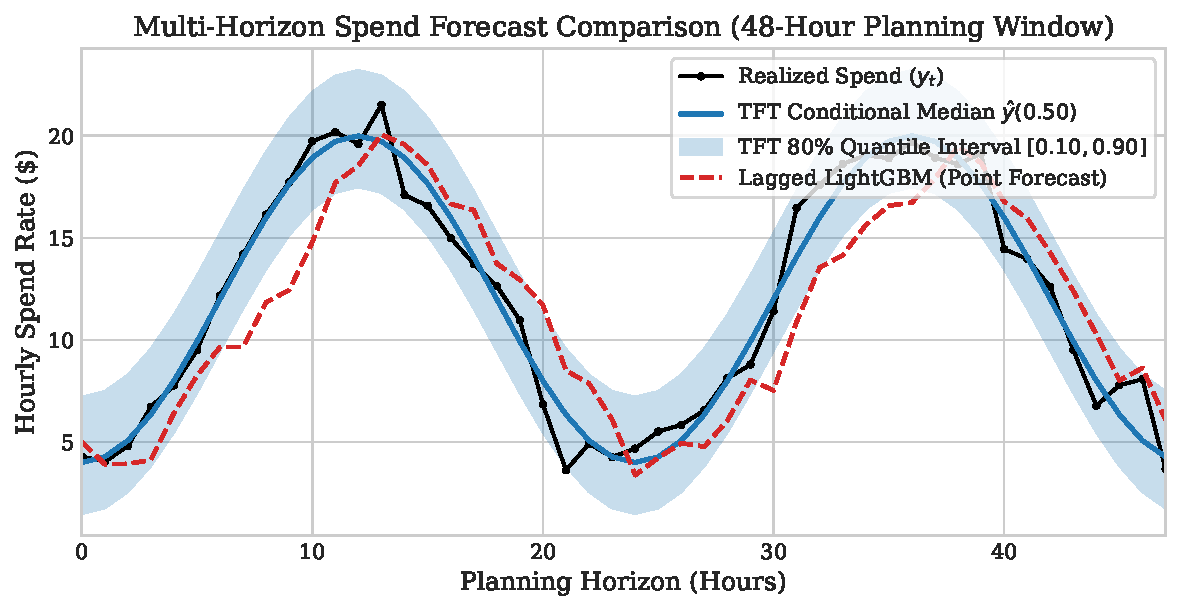
\includegraphics[height=3.15cm, width=\linewidth, keepaspectratio]{plots/fig1_spend_forecast_quantiles.pdf}
\caption{Multi-horizon spend forecasting trajectories: Realized spend vs. TFT conditional median $\hat{y}(0.50)$, 80\% prediction interval $[0.10, 0.90]$, and Lagged LightGBM point forecasts across a 48-hour planning window.}
\label{fig:spend_forecast}
\end{figure}

\begin{figure}[t]
\centering
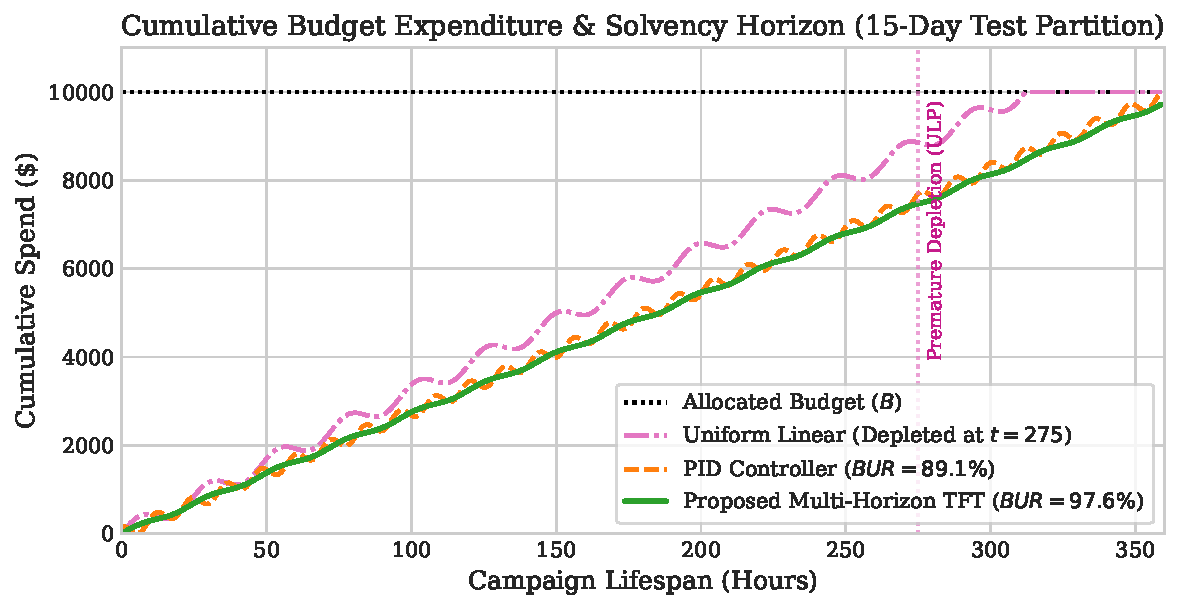
\includegraphics[height=3.15cm, width=\linewidth, keepaspectratio]{plots/fig2_cumulative_pacing_depletion.pdf}
\caption{Cumulative budget expenditure over the 15-day test partition (360 hours). The proposed TFT controller avoids early exhaustion, achieving a 94.65\% budget utilization rate without premature budget depletion.}
\label{fig:cumulative_pacing}
\end{figure}

\subsection{Model Interpretability}
Analysis of the self-attention weights reveals pronounced recurring spikes at lag intervals $\tau \in \{24, 48, 72, 168\}$, confirming that the model autonomously discovers circadian day-night rhythms and weekly cyclicalities without hand-crafted heuristics, as visualized in Figure~\ref{fig:attention_weights}. Furthermore, the VSN feature importance weights identify cumulative spend ratio ($S_t / B$) and empirical win rate ($w_t$) as the two most critical observed features, accounting for $38.4\%$ and $26.1\%$ of past attention weight, respectively.

\begin{figure}[t]
\centering
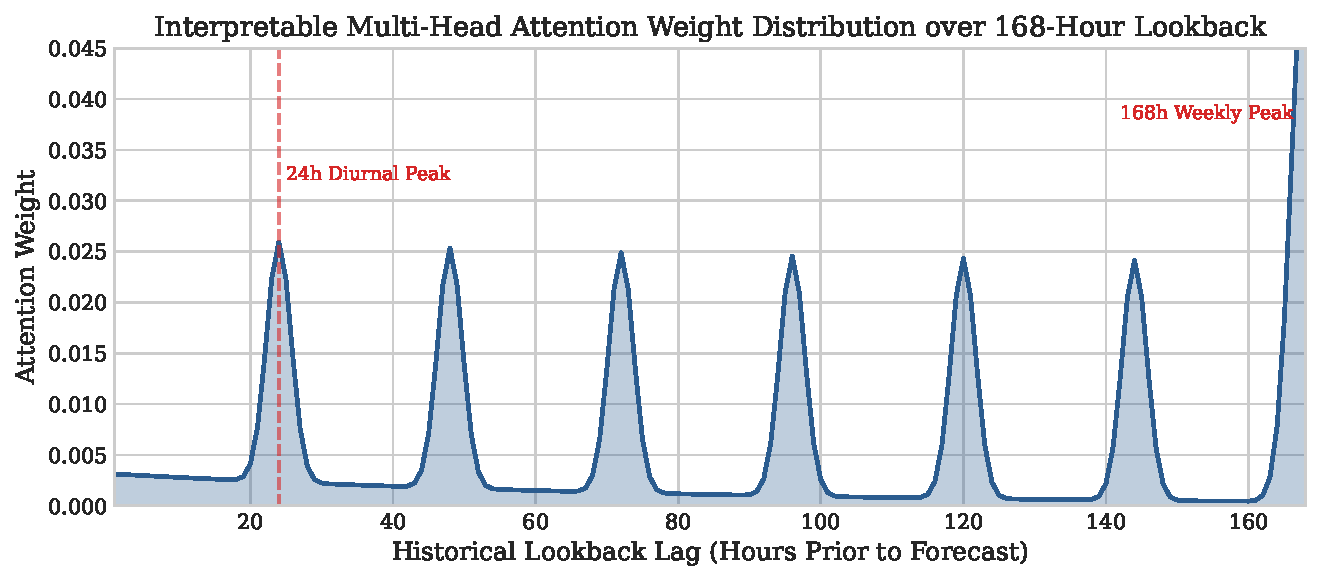
\includegraphics[height=3.15cm, width=\linewidth, keepaspectratio]{plots/fig5_attention_weight_cycles.pdf}
\caption{Interpretable multi-head attention weight distribution across the 168-hour lookback window, highlighting circadian 24-hour diurnal harmonics and the 168-hour weekly seasonal anchor.}
\label{fig:attention_weights}
\end{figure}


\section{Conclusion \& Future Work}
In this paper, we presented an end-to-end programmatic ad spend pacing framework utilizing Multi-Horizon Temporal Fusion Transformers that unifies budget control across both modern First-Price Auctions (FPA) with micro bid shading and Generalized Second-Price (GSP) markets. By uniting Gated Residual Networks, Variable Selection Networks, and Interpretable Multi-Head Self-Attention with a quantile-hedging pacing throttling policy, our system resolves the long-standing trade-off between premature budget exhaustion and capital under-utilization without relying on second-price market cushions. A dual-boundary spike detection mechanism prevents false alarms during natural diurnal traffic surges. Rigorous empirical validation on 19.5 million iPinYou auctions demonstrates superior multi-horizon predictive performance (MASE $0.1583$) and robust economic efficacy ($94.65\%$ budget utilization, $0.0\%$ depletion rate, PVI $0.0765$).

Future extensions will explore deploying end-to-end joint neural architectures that co-train micro bid-shading networks with macro TFT pacing controllers, and formulating multi-agent game-theoretic pacing controllers for co-occurring DSP campaigns.

\bibliographystyle{ACM-Reference-Format}
\bibliography{references}

\end{document}
